\documentclass{article}
\usepackage{url}
\usepackage{graphicx}
\usepackage{csvsimple}


\title{Master Thesis \\ Recommender Systems Comparison}
\date{27-05-2017}
\author{Vasileios Symeonidis}

\begin{document}
\maketitle
\newpage
\tableofcontents
\pagenumbering{gobble}
\newpage
\pagenumbering{roman}

\part{Master Thesis}
\newpage
\begin{center}
	This page was intentionally left blank.
\end{center}
\newpage
\chapter{Introduction}
\paragraph{} In the late 40s, a man called Alan Turing was investigating the case of a programmable computing machine. Of course, there were similar tries before. Babbage, for example, was famous for creating a computation machine. What made Turing's machine to differ? This machine was the first programmable one. I don't know how easily programmable you would call a machine in binary code, but at its time was the one. Turing prophetically enough said that we might need plenty of mathematicians of ability in order to program those machines.

\paragraph{} The years passed by, and lots of those machines appeared. The time was approaching for a general purpose, commonly supportive program that would take care of the trivial tasks. Tasks like standard input and output, and common program execution management. That kind of programs is called operating systems.

\paragraph{} Based on the previous advance the services provided by companies become more sophisticated. Services provided through software or provided using the software. To give an example, let us assume that we have a company A. This company specializes in delivering high-quality cars. After the operating systems introduction, this company has no need to make an operating system in order host an application that handles orders. This gave them the opportunity to low the cost of developing and maintaining a large part of their information system. Now, let's assume that we have a company B, this company specializes in consulting other companies on how to handle their orders. Either it does it through a software delivered to its customers or via a software for helping the company itself, an operating system truly changed their competitive advantage.

\paragraph{} The user provides data and actions. The application enhances the raw data provided by the user and persist them in a structured way, this could be for example a database, relational or not. If we take into account the above process, this means that the system has information about each user, his actions and the data he provided. This information is structured. Of course, the structure was made to serve the business cases of the application.

\paragraph{} The year is 1989, a British engineer working at CERN named Tim Berners-Lee invented the World Wide Web (W3). Of course, the first web site was on the world wide web which is somehow self-referential. W3 was mainly used by scientists in universities and institutes in order to share their work. 

\paragraph{}About a decade later, the RFC 1945: Hypertext Transfer Protocol - HTTP/1.0 \cite{berners1997rfc}, co-authored by Berners-Lee, was published, and W3 started to follow a more structured format.

\paragraph{} The last decade Internet has been flooded with information. Information that no one can manage to find what he needs. This information contains from raw data to videos, music or products. Large retail sites like Amazon developed recommenders systems in order to offer products to their users. The need although is not limited only in the retail area. 
\paragraph{}Web sites like Youtube or Vimeo need to recommend to each user of their, videos that may like to watch next. Facebook is another example of an application utilizing lots of data and offering recommendations on what you may want to read or who may be a friend of yours. Most of the times, a recommender system is not the core functionality of an application. It is through a very useful feature that gives a clear advantage in any business area needed.

\paragraph{}The way a recommender system has been built is very dependent on the business case which will be served. Even a specific case of recommendation, similar to one already existing, might need a different recommender system.

\paragraph{} So far recommender systems have been a very interesting area of study. Netflix in 2009 declared a challenge, which can be found here \footnote{http://www.netflixprize.com/}. Its reward was one million dollars for the task of improving the accuracy of predictions. The prize was granted to BellKor’s Pragmatic Chaos team for their algorithm. You can come across this challenge on lots of papers published every year.

\paragraph{} With such a wide study of recommender systems, it is reasonable to start wondering "How are we going to compare recommender systems?". As we will discuss below, there are several papers suggesting ways of comparison. The majority of those papers are using the dataset given in the challenge above.

\paragraph{} In this thesis, the first system to compare is a content-based recommendation system that provides predictions based on movies genre attributes. The second system is the based on the Alternating Least Squares (ALS) implementation of Apache Spark's MLlib.

\paragraph{} The comparison metrics used are the Mean Absolute Error (MAE), the Root Mean Squared Error and the ratio between them (MAE/RMSE). Last but not least is the execution of time metric, measuring the training and estimation time.

\newpage
\begin{center}
	This page was intentionally left blank.
\end{center}
\newpage
\chapter{Related Work}
\paragraph{} In this thesis's chapter, we will list numerous different approaches made in order to compare recommender systems.

\section{RecBench: Benchmarks for Evaluating Performance of Recommender System Architectures \cite{levandoski2011recbench}}
\paragraph{} The University of Minnesota, published in 2011 a paper stating a comparison between a recommender framework and a DBMS-based one. In that paper, they used the Movie Lens dataset 100k, from the Netflix Challenge. The benchmark had five areas of comparison. Those areas were initialization, pure recommendation, filtered recommendation, blended recommendation, item recommendation and item update.

\paragraph{}The initialization task was about the preparation needed for the system to go live. The next area was the pure recommendation. By pure recommendation, the author means the home page recommendation, meaning the items that are going to be on the homepage. Moving forward, we find the filtered recommendation. This recommendation is constrained by variables specific to the item, like movie genre etc. Another area of this evaluation contains the blended recommendation. Those recommendations are based on free text provided by the user in order to search. Item prediction is another area of the evaluation, in this prediction the user is navigated to the items page and the system is trying to predict the user's rating on the item. Last but not least, the paper examines the case of a new item being added to the system and how this is going to be incorporated into it.

\paragraph{}As a result, of those experiments, the paper concludes that "hand-build recommenders exhibit superior performance in model building and pure recommendation tasks, while DBMS-based recommenders are superior to more complex recommendations such as providing filtered recommendations and blending text-search with recommendation prediction issues.

\section{Recommender Systems Evaluation: A 3D Benchmark \cite{said2012recommender}}
\paragraph{}In this paper, the authors recognize the need for a common benchmark formula for recommender systems. This need leads them to propose one. They named it the 3D recommendation evaluation because they evaluate a system in three axes. These axes are business models, user requirements, and technical constraints. In business model axis they state that a recommender system must be evaluated on how well it serves the business case it is used for. In their paper, they give the example of a video on demand service and evaluate it versus the pay per view business model and pay per subscription.

\paragraph{}In the user requirements axis, the evaluate the system based on what needs it covers for the users. Is it, for example, going to reduce search time or decision-making time.

\paragraph{}Last but not least is the technical constraints axis. In this axis, the system is being evaluated based on data or hardware constraints, scalability, and robustness.

\section{RiVal: A New Benchmarking Toolkit for Recommender Systems \cite{said2014rival}}
\paragraph{} RiVal, is an open source toolkit implemented in Java programming language. Rival is available via Maven repositories. It is used in order to measure the evaluate recommender systems. Its evaluation is based on three points. Those points are data spitting, item recommendation, candidate item generation and performance measurement. 

\section{Collaborative filtering}
\subsection{Content based}
\subsection{Latent Factors}
test
sadsad

sad

asd

ds
\begin{figure}[ht]
\centering
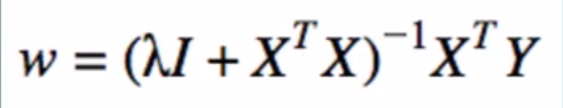
\includegraphics[width=0.7\linewidth]{images/equation01}
\caption{\bfseries Equation}
\label{fig:equation01}
\end{figure}

\section{Our Experiment}
\subsection{Infrastructure}
\subsubsection{Apache Spark}
\subsection{Dataset}
\subsection{Metrics}
\subsubsection{Mean Absolute Error}
\subsubsection{Execution Time}
\cite{ApacheSpark:1}
\cite{RecommenderSystems:2}
\cite{MovieLens:3}

\section{Results}
\begin{table}[ht]
		\caption {\bfseries Content Based Algorithm Results}
\begin{tabular}{l|l|r|r}%
   	\bfseries Training Dataset & \bfseries Testing Dataset & \bfseries Mean Absolute Error & \bfseries  Execution time (ms)% specify table head
   	\csvreader[head to column names]{data/contentBased.csv}{}% use head of csv as column names
   	{\\\hline \trainingSet & \testingSet & \MAE & \ExecutionTime}% specify your coloumns here
\end{tabular}
  \label{tab:Content Based Algorithm Results}
\end{table}

\begin{table}[ht]
		\caption{\bfseries Latent Factors Algorithm Results}
\begin{tabular}{l|l|r|r}%
	\bfseries Training Dataset & \bfseries Testing Dataset & \bfseries Mean Absolute Error & \bfseries  Execution time (ms)% specify table head
	\csvreader[head to column names]{data/latentFactors.csv}{}% use head of csv as column names
	{\\\hline \trainingSet & \testingSet & \MAE & \ExecutionTime}% specify your coloumns here
\end{tabular}
  \label{tab:Latent Factors Algorithm Results}
\end{table}


\section{Conclusion}
\section{references}

\newpage
\appendix
\part{Appendices}
\section{Code used}
\subsection{User Based Collaborative Filtering}
\subsection{Product Based Collaborative Filtering}
\subsection{Latent Factors}
\section{infra code}
\section{Metrics}
\subsection{What is the mean absolute error}
\subsection{Time}
\newpage
\listoffigures


\section{List of Tables}
\listoftables
\newpage
\bibliography{thesis}
\bibliographystyle{ieeetr}
%\footnote{}
%\cite{DUMMY:1}
%https://www.sharelatex.com/learn/Lists_of_tables_and_figures
\end{document}
